\chapter{Results}

%A concept will be developed on how a model for predicting user intent could be built and how it could be applied to the user session.
%To this end, possibilities for collecting and vectorizing sequential UI trees will be discussed
%which are designed to predict the user intent. Here, privacy and feature pre-filteringin UI data plays an important role
%
%After that, personalized as well as collaborative data can be used in a hybrid approach.
%This modelshould then be made available to the user in an Android app service and, depending on the level ofdetail, suggest upcoming apps or actions to the user at a suitable time

This chapter will explain how a prediction model for user intent can be designed and what factors of influence have to be considered.
The design will be shown on the basis of a proof of concept implementation.
Also, a concept of how this model can be applied to the real world is proposed. \todo{check if that is actually done.}

As noted in the introduction the term \ti{intent} has a very wide scope.
It's prediction can only be made in fractions, or serve as indicator.
The semantically closest way and also the most detailed would be to describe the users intent in words, thus a description of what the user wants to do next.
Unfortunately, the users intent description cannot be determined yet, as no according dataset is provided.
An important step, the screen summarization as shown in Screen2words~\ref{subsec:screen2words}, already was made, which could also be fed with the users intention descriptions.
But this would then only reflect the already passed fulfilled intent and not the upcoming next purpose.
Also, the users flows can be predicted as shown in the works of ERICA~\ref{subsec:erica}.
\todo{may more describe what a 'flow' can do}
Next app prediction already works quite well~\ref{todo}, which also reflects the larger intent of the user, but is not very detailed.

In order to approximate that goal the assumption was made that the next \tb{user interaction} also give hints on what the user is intending to achieve.
The interaction is resulting in another screen, which then the user (hopefully) intends to see.


Proof of concept, as an example gesture or click traces were used as labels.
More general approaches can be used such as a description of the intent \cite{wang2021screen2words}, which needs another data set.

%\todo{overall goal is more than just interaction traces}
Make the algorithm as independent of the data as possible.
Find general rules to feed the data.
Applicable to other research fields, not just UI traces.
Use LSTM, so predict something unseen, in contrast to RICO or ERICA, which only categorize the current context

%Steps:
%- Data acquisition
%- Data cleaning / Preprocessing (Panadas)
%- Split into Training Data, Validation data, and Test data (cannot adapt the model after using the test data)
%- Train the model with the train data
%- Evaluate the model with the test data, then can adapt the model by the developer
%- Last deploy the model to production

\section{Datasets}

- Problem with sequential data sets
- Google and Samsung
- need to have correct data
- no missing data
- needs enough data to train a NN
- need enough features to be able to recognize patterns
- up to date
- Publicly available
- Variable length of app sessions, define one session of activating the screen until it is turned off.

Missing
- System to feed in in real time
- Dataset which is across multiple apps, also tracks the system
-

\subsection{Rico}

\begin{itemize}
  \item Too less frames.
  \item No transition between apps.
\end{itemize}

\section{Preprocessing Android UI tree data}
\subsection{Filtering privacy invasive details}

- rico doesn't use logins or any privat data
- gestures can tell more about the user
-


\subsection{Normalization, Feature Selection}

Dealing with variable length data tf.io.VarLenFeature()

\section{Model}

%- Screen2Words

LSTM 4 dimensional
% https://stackoverflow.com/questions/54743549/is-it-possible-to-making-lstm-model-with-4-dimension-shape-of-data

Limitations to only 3 dimensions, needs flattening

Sample dimension (X -> y)
Time (Step) Dimension
Feature Dimension
Data, Quantity dimension, such as Image dimensions, or multiple nodes

TimeDistributedLayer
% https://stackoverflow.com/a/61588937/5164462
% https://stackoverflow.com/questions/53107126/what-are-the-uses-of-timedistributed-wrapper-for-lstm-or-any-other-layers


Multiple approaches

\todo{create graphic for each approach}

AutoEncoder:

\begin{itemize}
  \item Encoder -> Decoder -> LSTM -> Decoder
  \item Encoder -> LSTM -> Decoder
  \item LSTM -> Encoder -> Decoder (AutoEncoder)
\end{itemize}

Decoder can either only decode to x and y or to whole UI tree.

\section{Evaluation}

\begin{figure}[htbp!]
  \centering
  \begin{subfigure}[b]{0.45\textwidth}
    \centering
    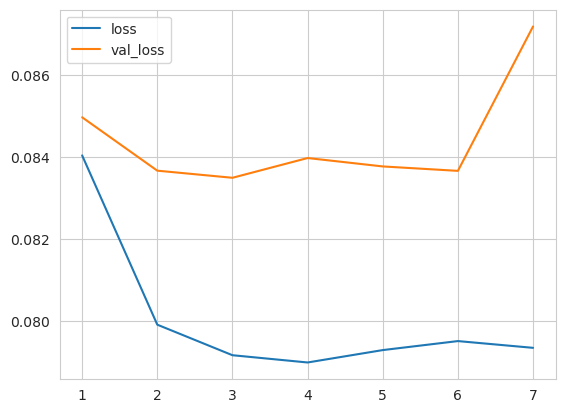
\includegraphics[width=\textwidth]{graphics/model_history_loss_clicks}
    \caption{Clicks as features only}
    \label{fig:model_history_loss_clicks}
  \end{subfigure}
  \hfill
  \begin{subfigure}[b]{0.45\textwidth}
    \centering
    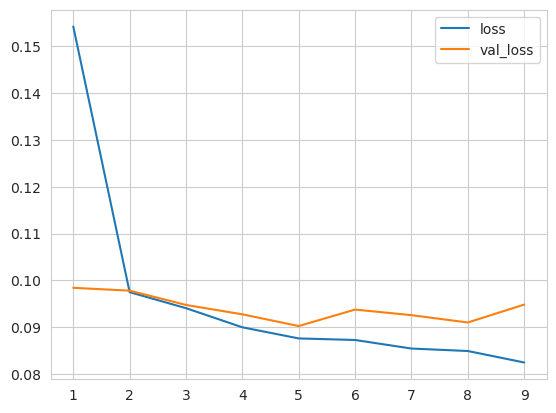
\includegraphics[width=\textwidth]{graphics/model_history_loss_features}
    \caption{Bounding box and click features}
    \label{fig:model_history_loss_features}
  \end{subfigure}
  \hfill
  \begin{subfigure}[b]{0.8\textwidth}
    \centering
    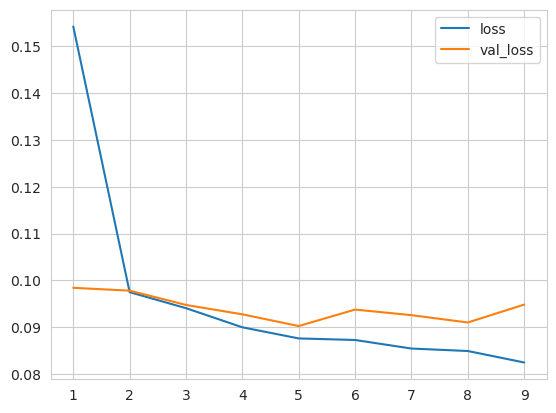
\includegraphics[width=\textwidth]{graphics/model_history_loss_features}
    \caption{Bounding box and shifted click features}
    \label{fig:model_history_loss_features_shifted}
  \end{subfigure}
  \caption[Training loss vs. validation loss]{Training loss vs. validation loss.}
  \label{fig:model_history_losses}
\end{figure}

\subsection{Mean Squared Error}

\section{Limitations}

Dataset
Dataset is not through different apps, only in one app.
Dataset is not detailed enough in the time steps, or not containing all data
Dataset is not long enough
Dataset has no paid apps or apps with login, which most services require
Dataset has wrong data see \cite{clay}

Preprocessing
Need more time to validate what are the core parameters to predict the next user intent


Model needs more investigation on what data is needed
How many neurons are required to achieve this
Play around with different layers, also Convolutional and pretrained embeddings

